% !TEX encoding = UTF-8 Unicode

\documentclass[a4paper]{article}

\usepackage{color}
\usepackage{url}
\usepackage[T2A]{fontenc} % enable Cyrillic fonts
\usepackage[utf8]{inputenc} % make weird characters work
\usepackage{graphicx}
\graphicspath{{slike/}}
\usepackage{listings}
\usepackage{changepage}
\usepackage{amsmath}

\usepackage[english,serbian]{babel}

\usepackage[unicode]{hyperref}
\hypersetup{colorlinks,citecolor=green,filecolor=green,linkcolor=blue,urlcolor=blue}

\newtheorem{primer}{Primer}[section]

\begin{document}
	
	\title{Paralelno programiranje\\ \small{Seminarski rad u okviru kursa\\Tehničko i naučno pisanje\\ Matematički fakultet}}
	
	\author
	{
		Aleksandar Đukić\\mi22144@alas.matf.bg.ac.rs
		\and
		Iva Minić\\mi22153@alas.matf.bg.ac.rs
		\and
		Luka Mitrović\\mi22092@alas.matf.bg.ac.rs
		\and
		Marija Zrnić\\mi22293@alas.matf.bg.ac.rs
	}
	
	\date{13.~novembar 2022.}
	\maketitle
	
	\abstract{
		Ovde ide tekst ovde ide tekst ovde ide tekst ovde ide tekst ovde ide tekst ovde ide tekst ovde ide tekst ovde ide tekst ovde ide tekst ovde ide tekst ovde ide tekst ovde ide tekst ovde ide tekst ovde ide tekst
		}
		\tableofcontents
		
	\newpage
	\section{Uvod}
	Ovde ide tekst ovde ide tekst ovde ide tekst ovde ide tekst ovde ide tekst ovde ide tekst ovde ide tekst ovde ide tekst ovde ide tekst ovde ide tekst ovde ide tekst ovde ide tekst ovde ide tekst ovde ide tekst
	
	\section{Istorija}
	Da bi se pričalo o istoriji paralelnog programiranja, potrebno je prvo pričati o istoriji paralelne obrade.
	\subsection{Istorija paralelne obrade}
	Koreni paralelne obrade nalaze se u 1950-im godinama. Dva zaposlena iz IBM (en. International Business Machines Corporation), Džon Kok i Daniel Slotnik, prvi put diskutuju paralelizam u radu koji su zajedno objavili 1958 \cite{historyofdevelopment}. Tokom narednih godina, razne firme počinju rad na razvoju mašina sposobnih za paralelnu obradu. 1962, korporacija Burroughs proizvodi ~{\em D825 Modular Data Processing System} — računar razvijen za rad u vojnom okruženju \cite{d825}. Zbog njegove namene, on radi po principu SMP (eng. symmetric multiprocessing ili shared-memory multiprocessing) - dva ili više procesora su povezana na zajedničku memoriju, i kontroliše ih isti operativni sistem. U slučaju D825, koriste se 4 centralne procesorske jedinice, koje imaju pristup do 16 modula memorije \cite{d825}. D825 se smatra prvim pravim multiprocesorskim računarom \cite{multiprocessororganizationsurvey}.\par
	Na Spring Joint konferenciji Američke federacije društva za obrađivanje podataka (eng. American Federation of Information Processing Societies, AFIPS), održane 1967, Daniel Slotnik i Džin Amdal debatovali su o paralelnoj obradi \cite{springjoint}. U ovoj debati nastaje Amdalov zakon ili Amdalov argument, koji opisuje granicu efikasnosti paralelne obrade. Ovaj zakon će se često koristiti da bi se predvidila efikasnost i vreme izvršavanja paralelizovanog programa.\par
	Priča o računarskim sistemima sa raspodeljenom memorijom  (eng. distributed memory) započinje 1960-ih, ali se prvi takav računar pojavljuje tek 1983\cite{hypercube}. \emph{The Cosmic Cube} od instituta \emph{Caltech} sadrži 64 procesora koji istovremeno rade na jednom problemu, i međusobno komuniciraju tako što jedan drugome šalju poruke\cite{thecosmiccube}.
	\subsection{Istorija paralelnog programiranja}
	Uz razvoj paralelne obrade, počeo je da se pojavljuje veliki broj interfejsa koji su se do 1990-ih ujedinili u nekoliko standarda. 1992. održana je radionica na temu standarda za razmenu poruka u okruženju sa raspodeljenom memorijom (eng. Standards for Message-Passing in a Distributed Memory Environment) \cite{standardsformessagepassing}, na kojoj je započet razvoj standarda koji će se 1994. objaviti pod nazivom MPI (eng. Message Passing Interface). Naknadno su objavljeni standardi MPI 2.0 (1996), MPI 3.0 (2012) i MPI 4.0 (2021)\cite{mpidocs}.\par
	Sa druge strane, za programiranje u SMP okruženju, OpenMP ARB (Architecture Review Board) objavljuje prve specifikacije interfejsa OpenMP 1.0 za Fortran u 1997, a sledeće godine i standard za C/C++. Nakon toga, objavljene su i verzije OpenMP 2.0 (2007), 3.0 (2008), 4.0 (2013) i 5.2 (2021), koji se koristi danas\cite{opemp5}.
	
	\section{Princip rada paralelnog programiranja}
	Opšte rečeno, paralelno programiranje radi tako što deli program na više zadataka koji se izvršavaju istovremeno. Da bi bolje razumeli celu sliku, moramo prvo objasniti paralelnu obradu.
	\subsection{Osnove paralelne obrade}
	Paralelna obrada predstavlja sva izračunavanja na računaru koja se izvršavaju paralelno, tj. istovremeno \cite{p98}. Postoje više formi paralelne obrade, od kojih su najvažnije prikazane u narednoj tabeli:\\

	
\begin{adjustwidth}{-2cm}{}
\begin{tabular}{|c|c|c|}
\hline
Naziv                                                                                  & Opis                                                                                                                                                                                                                                                                                                           & Mane                                                                                                                                                                                   \\ \hline
\begin{tabular}[c]{@{}c@{}}Nivo bita\\ (eng. bit-level)\end{tabular}                   & \begin{tabular}[c]{@{}c@{}}Zasniva se na proširenju  veličine \\ procesorske reči (osnovna jedinica podataka \\ koju koristi određeni  dizajn procesora). \\ Koristi se u slučaju kada je broj bitova \\ podatka kojeg je potrebno obraditi \\ veći nego što procesor podržava za jednu\\ obradu.\end{tabular} & \begin{tabular}[c]{@{}c@{}}Trošak vremena i hardvera, \\ tehnike eksploatacije ne \\ ostvaraju pun potencijal\end{tabular}                                                             \\ \hline
\begin{tabular}[c]{@{}c@{}}Nivo naredbe\\ (eng. instruction level)\end{tabular}        & \begin{tabular}[c]{@{}c@{}}Predstavlja istovremeno \\ izvršavanje niza naredbi. \\ Daje prosečan broj naredbi koje\\ se izvršavaju pri svakom \\ koraku paralelne obrade \cite{ILP}.\end{tabular}                                                                                                                         & \begin{tabular}[c]{@{}c@{}}Ograničeno od zavisnosti \\ kontrole i podataka\end{tabular}                                                                                                \\ \hline
\begin{tabular}[c]{@{}c@{}}Paralelizam podataka\\ (eng. data parallelism)\end{tabular} & \begin{tabular}[c]{@{}c@{}}Deli podatke na više procesora \\ tako da se nad njima vrši \\ isti zadatak istovremeno \cite{dataandtaskparallel}.\end{tabular}                                                                                                                                                                               & \begin{tabular}[c]{@{}c@{}}Mogu nastati problemi tokom\\  nepravilne manipulacije podacima, \\ ograničeno je sa količinom \\ podataka koji mogu da\\ protiču iz memorije.\end{tabular} \\ \hline
\begin{tabular}[c]{@{}c@{}}Paralelizam zadataka\\ (eng. task parallelism)\end{tabular} & \begin{tabular}[c]{@{}c@{}}U kontrastu sa paralelizmom podataka, \\ ovde se dele zadaci koji \\ se izvršavaju nad \\ jednim podatkom istovremeno \cite{dataandtaskparallel}.\end{tabular}                                                                                                                                                 & \begin{tabular}[c]{@{}c@{}}Ograničeno troškovima \\ komunikacije i sinhronizacije\end{tabular}                                                                                         \\ \hline
\end{tabular}\\
\end{adjustwidth}

Mane formi iz tabele i činjenica da se paralelizam često koristi zajedno sa sekvencijalnim programiranjem postavljaju pitanje, koliko je potencijalno ubrzanje izvršavanja zadataka ako primenimo paralelizam? Ovime se bavi ranije pomenut Amdalov zakon, koji meri efikasnost izvršavanja paralelnog programa. On kaže da celokupan dobitak zavisi od količine vremena prilikom kojeg se zapravo koristi paralelnost: \\
\begin{equation*}
S_{max} = \frac{1}{(1 - p) + \frac{p}{s}}
\end{equation*}\\
$S_{max}$ je maksimalna potencijalna efikasnost, $p$ procenat sistema koji je poboljšan, a $s$ deo vremena u kojem radi poboljšani deo sistema. Kada bi se ova formula primenila na moderne računare, naizgled bi paralelnost bila nedovoljno efikasna, ali to nije slučaj. Ovo je primetio Džon Gustafson i ponovo ispitao Amdalov zakon i došao do svog zaključka, koji prikazuje efikasnost paralelizma tako što upoređuje rad istog zadatka na mašini sa jednim jezgrom:\\
\begin{equation*}
S_{max} = N + (1 - N) * s
\end{equation*}\\
Gde je $S_{max}$ maksimalna potencijalna efikasnost, $N$ broj procesora koji obrađuje podatke, a $s$ vreme za koje se zadatak obradi sekvencijalno.
\subsection{Koraci paralelizacije programa}
Sada kada znamo principe paralelne obrade, možemo komentarisati o koracima koji vode do kreiranja paralelnog programa. To su: dekompozicija, dodela, orkestracija i mapiranje.\par
Dekompozicija prvo razdvaja obradu na više zadataka koji se kasnije dele među procesima. Traži paralelizam i koliko može da ga iskoristi. Cilj je kreirati dovoljno zadataka da bi ih procesori istovremeno izvršavali, pri čemu zadaci mogu nastajati dinamički i njihov broj može da varira.\par 
Kod dodele se određuje mehanizam koji deli zadatke iz prethodnog koraka među procesima. Cilj je da balansira rad, a i smanji troškove komunikacije i menadžmenta. Zajedno sa dekompozicijom ova dva koraka su poznata kao particionisanje, tj. raspodela više različitih zadataka na više procesa. \par 
Orkestracija smanjuje trošak komunikacije i sinhronizacije, imenuje podatke, čuva strukture podataka i njihove lokalne reference, organizuje rad, pravi raspored izvršavanja zadataka tako da ne dođe do preopterećenja ili manjka zadataka koji se trenutno izvršavaju. \par 
Nakon ovog koraka, već imamo paralelni program, ali mapiranje je tu da reguliše koji procesi će biti izvršavani na istom procesoru, kao i koji procesi će se izvršavati na nekom specifičnom procesoru generalno. 
\subsection{Modeli paralelnog programiranja}
Termin komunikacija se često pominje tokom koraka paralelizacije, a on se zapravo odnosi na razmenjivanje podataka između procesa koji se trenutno izvršavaju \cite{models}. Na osnovu ovoga nastalo je nekoliko modela, od kojih su najvažniji: \\
\begin{itemize}
\item Model deljene memorije (eng. shared memory model) - Kod ovog modela svi procesi imaju pristup jednom glavnom delu programa koji sadrži sve podatke. Procesi mogu asinhrono da čitaju i pišu u ovoj međusobno deljenoj memoriji. Ipak, zbog toga mogu nastati problemi kao što je data race, o čemu će biti reči kasnije.
\item Model prenošenja poruke (eng. message passing model) - U ovom modelu, procesi koji se paralelno izvršavaju šalju jedni drugima podatke preko poruka, koje mogu biti asinhrone (primalac dobija poruku i da nije spreman na to) i sinrhone (obe strane su u trenutku slobodne da pošalju i prime poruku).
\item Particionisani globalni adresni prostor (eng. partitioned global address space) - Model koji je hibrid prethodna dva, gde se koristi deljena memorija, međutim ovaj put je ona particionisana tako da svaki proces ima pristup samo određenim tačkama u memoriji, umesto celokupnom prostoru. Podaci se razmenjuju pisanjem i čitanjem iz datog dela memorije.
\end{itemize}
	
	\section{Upotrebe}
Sada kada znamo šta je paralelno programiranje možemo da pričamo o tome gde i kada se koristi.
\subsection{Osnovne primene}

Paralelno programiranje koristimo kada imamo velike količine podataka, kompleksne račune ili velike simulacije. Iako paralelno programiranje može biti vremenski intenzivniji napor za programere da kreiraju efikasne paralelne algoritme i kod, ono sveukupno štedi vreme tako što koristi pun potencijal procesora.\\Neke od oblasti u kojima paralelno programiranje može biti korisno su: primenjena fizika, elektrotehnika, finansijsko i ekonomsko modeliranje,  nacionalna bezbednost i nuklearno oružije, veštačka inteligencija, kvantna mehanika\cite{totalview} i još mnoge druge.

\subsection{Prednosti i mane}

Prednosti paralelnog programiranja su:
\begin{itemize}
\item \textbf{Brzina} - Možemo postići bolje performanse jer su zadaci raspoređeni u nitima koje rade paralelno.\cite{zoboko}
\item \textbf{Poboljšan GUI} - Pošto zadaci obavljaju neblokirajući I/O, to znači da je GUI nit uvek slobodna da prihvati korisničke unose. Ovo dovodi do boljeg odziva.\cite{zoboko}
\item \textbf{Istovremeno i paralelno pojavljivanje zadataka koji se pokreću paralelno} - Možemo istovremeno pokrenuti različite logike programiranja.\cite{zoboko}
\item \textbf{Bolje korišćenje keš memorije korišćenjem resursa i bolje korišćenje CPU resursa} - Zadaci se mogu izvršavati na različitim jezgrima, čime se obezbeđuje maksimalna propusnost.\cite{zoboko}\\
\end{itemize}
Mane:
\begin{itemize}
\item \textbf{Promena konteksta} - svaka nit radi na delu vremena koji joj je dodeljen. Kada vremenski odlomak istekne, dešava se promena konteksta, što takođe troši resurse.\cite{zoboko}
\item \textbf{Nepredvidljivost} - pošto se paralelno programiranje oslanja na CPU jezgra, možemo dobiti različite rezultate na različitim konfigurisanim mašinama.\cite{zoboko}
\item \textbf{Teško za programiranje} - paralelne programe može biti teško napisati u poređenju sa sinhronim verzijama.\cite{zoboko}
\item \textbf{Kompleksno otklanjanje grešaka i testiranje} - korišćenje više niti pomaže da dobijete više od jednog procesora. Ali onda ove niti treba da sinhronizuju svoj rad u zajedničkoj memoriji. Ovo može biti teško ispraviti - a još teže bez problema sa istovremenošću\cite{zoboko}.
Evo dve uobičajene vrste problema sa više niti koje može biti teško pronaći samo testiranjem i otklanjanjem grešaka:
\begin{enumerate}
\item \textbf{Data Race} - 
Data race nastaje kada dve ili više niti pristupaju deljenjim podacima i pokušavaju da ih modifikuju u isto vreme bez odgovarajuće sinhronizacije. Ova vrsta greške može dovesti do kvarova ili oštećenja memorije.\cite{perforce}
\item \textbf{Deadlock} - 
Deadlock se javlja kada je više niti blokirano dok se takmiče za resurse. Jedna nit je zaglavljena čekajući drugu nit, koja je zaglavljena čekajući prvu. Ova vrsta greške može dovesti do zaglavljivanja programa.\cite{perforce}
\end{enumerate}
\end{itemize}

	
	\section{Primeri}
    Danas većina programskih jezika podržava paralelno programiranje, ali, radi jednostavnosti i čitljivosti, koristićemo programski jezik Python. Uz Python standardnu biblioteku dolazi i modul \emph{multiprocessing}, koji omogućava paralelno pokretanje više procesa.
    \subsection{Primer 1 - Preuzimanje sadržaja u pozadini}
    Jedna od najčešćih upotreba paralelnog programiranja je izvršavanje neke operacije u pozadini, dok glavni program nesmetano nastavlja sa radom. 
    \par U ovom primeru prikazan je program koji kreira novi proces, i pomoću njega preuzima prvih 20 cifara broja pi sa određene internet adrese i ispisuje ih. Za to vreme glavni proces nastavlja normalno sa radom.
    \begin{lstlisting}[showstringspaces=false, language=Python]
    p = multiprocessing.Process(target=download_pi)
    p.start()
    while (True):
        print("Glavni proces...")
        time.sleep(0.5)
    \end{lstlisting}
    U prvoj liniji koda kreira se proces \emph{p} - objekat klase \lstinline{Process}. Kao argument šaljemo naziv procedure koju proces treba da izvrši. I konačno ga pokrećemo metodom \lstinline{start()}. Program neće čekati da se izvršavanje okonča, nego će nastaviti normalnim tokom. U naredne 3 linije nalazi se petlja koja će da ispisuje određeni tekst na svakih pola sekunde. Ovaj deo postavljen je kako bi prikazao da se procesi izvršavaju paralelno.
    \par Definicija procedure \lstinline{download_pi} koju proces izvršava:
    
    \begin{lstlisting}[showstringspaces=false, language=Python]
    def download_pi():
        req = requests.get("https://api.pi.delivery/v1/
                            pi?start=0&numberOfDigits=20")
        req = req.json();
        print("Prvih 20 cifara broja pi:", req["content"])
    \end{lstlisting}
    \par Rezultat pokretanja celog programa:
    \begin{lstlisting}[showstringspaces=false, language=Python]
    Glavni proces...
    Glavni proces...
    Prvih 20 cifara broja pi: 31415926535897932384
    Glavni proces...
    ...
    \end{lstlisting}
    Vidimo da je paralelizacija uspela, jer bi se u suprotnom prvo završilo izvršavanje procedure \lstinline{download_pi}, pa tek onda program nastavio s radom.
    \subsection{Primer 2 - Broj prostih brojeva u listi}
    Nekada je za jedan problem potrebno pokrenuti više procesa. To su obično izuzetno zahtevne komputacije, kao što je, na primer, kriptografija ili kompresija velike količine podataka, ili kompilacija koda. Iako možemo pokrenuti više procesa pojedinačno (slično prethodnom primeru), \emph{multiprocessing} pruža mogućnost korišćenja klase \lstinline{Pool}. 
    \par \lstinline{Pool} predstavlja skup procesa koji će izvršavati isti zadatak. Prilikom inicijalizacije, potrebno je proslediti samo broj procesa, koji ne može biti veći od broja jezgara na procesoru.
    \par U ovom primeru prikazan je program koji izračunava broj prostih brojeva u nekoj listi brojeva.
    \begin{lstlisting}[showstringspaces=false, language=Python]
    pool = multiprocessing.Pool(processes=4)
    nums_list = generate_list(15000, 9, 12)
    nums_list = chunks(nums_list, 4)
    print(sum(pool.map(count_primes, nums_list)))
    \end{lstlisting}
    \par U prvoj liniji kreiramo \lstinline{pool}, koji će sadržati 4 procesa.
    Dalje, generišemo listu \lstinline{nums_list} (pomoću procedure \lstinline{generate_list}), koja će sadržati 15000 nasumičnih brojeva u intervalu $\left [ 10^{9}, 10^{12} \right ]$. 
    \par S obzirom da se, pri kreiranju procesa, oni ``odvajaju'' od glavne memorije programa, potrebno je proslediti im podatke na kojima će vršiti komputacije. Da bi program bio što efikasniji, treba podeliti podatke na približno jednake delove. Delova bi trebalo biti onoliko koliko i procesa.
    U ovom slučaju, koristićemo proceduru \lstinline{chunks}, koja će listu podeliti na 4 približno jednaka dela, i vratiti novu listu koja sadrži te 4 podliste.
    \par U poslednjoj liniji koristimo metodu \lstinline{map()}, i prosleđujemo joj proceduru \lstinline{count_primes} i listu \lstinline{nums_list}. Ova metoda će u svakom procesu (koji se nalazi unutar skupa \lstinline{pool}) pozvati proceduru \lstinline{count_primes}, dok će kao argument proslediti jedan od elemenata liste \lstinline{nums_list}, odnosno jedan od one 4 podliste. Nakon što svaki od procesa okonča izvršavanje, upisaće rezultat koji dobije u novu listu, koja će imati isto onoliko elemenata koliko i \lstinline{nums_list}, odnosno 4. Procedura \lstinline{sum} sabraće sve elemente novodobijene liste, a \lstinline{print()} će dobijeni zbir ispisati.
    \subsection{Poređenje performansi}
    Sada ćemo testirati efikasnost paralelnog programiranja. Za to ćemo iskoristiti poslednji primer - brojanje prostih brojeva u listi. Uporedićemo vreme izvršavanja sa 1, 2, 4, 8 i 12 paralelnih procesa.
    \par Da bi merili vreme izvršavanja, potrebna je samo jedna mala izmena u kodu. Pomoću metode \lstinline{time.time()}, sačuvaćemo vremenski trenutak pre početka izvršavanja glavnog zadatka. Zatim to isto uraditi i tačno nakon izvršenja. Razlika ta dva vremenska trenutna predstavlja vreme izvršavanja zadatka.
    \begin{lstlisting}[showstringspaces=false, language=Python]
    start = time.time()
    print(sum(pool.map(count_primes, nums_list)))
    print(time.time() - start)
    \end{lstlisting}
    Za 5000 nasumičnih brojeva u intervalu $\left [ 10^{9}, 10^{12} \right ]$, i 4 procesa koja izvršavaju zadatak, rezultat je sledeći:
    \begin{lstlisting}[showstringspaces=false, language=Python]
    203
    6.540586948394775
    \end{lstlisting}
    \par Vreme je prikazano u sekundama. 
    \begin{figure}[h]
    \caption{Brzina izvršavanja u odnosu na broj procesa}
    \begin{center}
    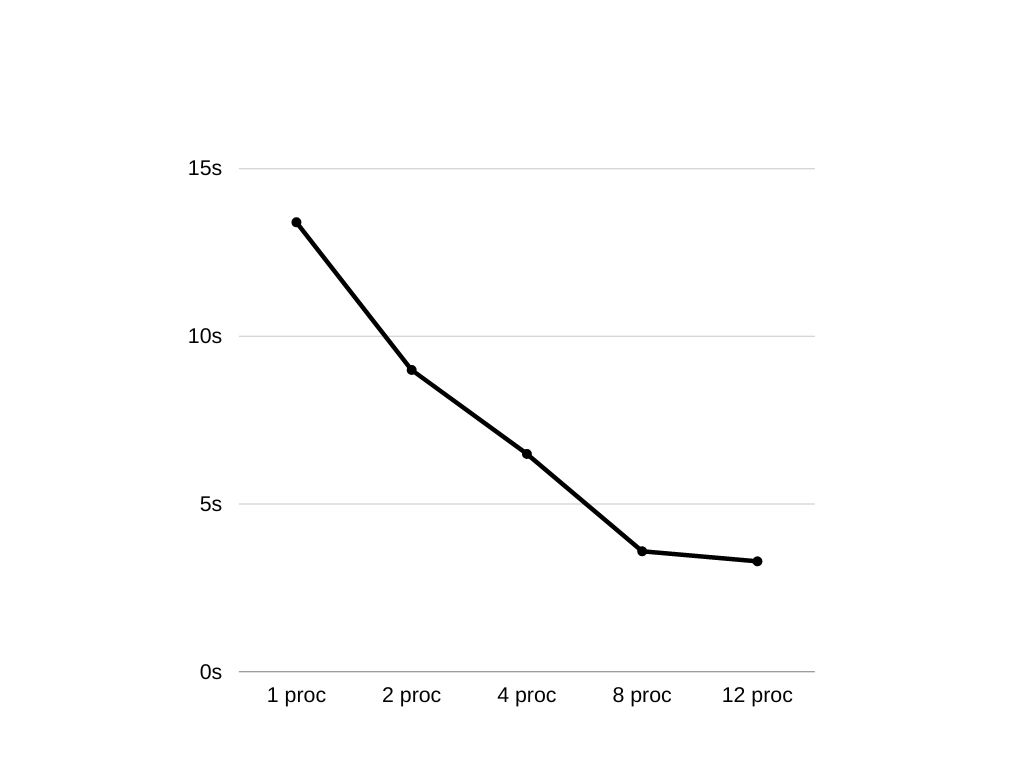
\includegraphics[scale=0.3]{grafik}
    \end{center}
    \par Na slici iznad prikazane su brzine izvršavanja u odnosu na broj procesa. Može se primetiti da je program efikasniji što više procesa koristi.
    \end{figure}
	
	\section{Zaključak}
	\label{sec:zakljucak}
	Ovde pišem zaključak. 
	Ovde pišem zaključak. 
	Ovde pišem zaključak. 
	Ovde pišem zaključak. 
	Ovde pišem zaključak. 
	Ovde pišem zaključak. 
	Ovde pišem zaključak. 
	Ovde pišem zaključak. 
	Ovde pišem zaključak. 
	Ovde pišem zaključak. 
	Ovde pišem zaključak. 
	Ovde pišem zaključak. 
	
	\addcontentsline{toc}{section}{Literatura}
	\appendix
	
	\iffalse
	\bibliography{seminarski} 
	\bibliographystyle{plain}
	\fi
	
	\begin{thebibliography}{50}
		
		\bibitem{historyofdevelopment} G. V. Wilson. \emph{The History of the Development of Parallel Computing}. CS Dept. NSF-Supported Education Infrastructure Project, 1994. on-line at: https://ei.cs.vt.edu/~history/Parallel.html
		
		\bibitem{d825} J. P. Anderson, S. A. Hoffman, J. Shifman, and R. J. Williams. \emph{D825 — A Multiple-Computer System For Command \&Control}. Burroughs Corporation, Pennsylvania, 1962.
		
		\bibitem{multiprocessororganizationsurvey} P. H. Enslow Jr. \emph{Multiprocessor Organization — A Survey}. School of Information and Computer Science, Georgia Institute of Technology, Atlanta, Georgia, USA, 1977.
		
		\bibitem{springjoint} Proceedings of the April 18-20, 1967, spring joint computer conference. Association for Computing Machinery, New York, NY, USA, 1967.
		
		\bibitem{hypercube} G. Ostrouchov. \emph{Parallel Computing on a Hypercube: An Overview of the Architecture and Some Applications}. Oak Ridge National Laboratory, USA, 1987.
		
		\bibitem{thecosmiccube} C. L. Seitz. \emph{The Cosmic Cube}. California Institute of Technology. California, USA, 1985.
		
		\bibitem{standardsformessagepassing} D. W. Walker. \emph{Standards For Message-Passing in a Distributed Memory Environment}. Mathematical Sciences Section Oak Ridge National Laboratory, Tennessee, USA, 1992.
		
		\bibitem{mpidocs} \emph{MPI forum}. https://www.mpi-forum.org/docs/, 13. 11. 2022.
		
		\bibitem{opemp5} \emph{The OpenMP API specification for parallel programming}. https://www.openmp.org/specifications/, 14. 11. 2022.
		
		\bibitem{totalview} \emph{TotalView: What Is Parallel Programming?} https://totalview.io/blog/what-is-parallel-programming, 17. 11. 2022.
		
		\bibitem{perforce} \emph{Perforce: What Is Parallel Programming and Multithreading (Multithreaded Programming)?} https://www.perforce.com/blog/qac/multithreading-parallel-programming-c-cpp, 17. 11. 2022.
		
		\bibitem{zoboko} Shakti Tanwar. \emph{Hands-On Parallel Programming with C\# 8 and .NET Core 3: Build solid enterprise software using task parallelism and multithreading}, 2019.
		
		\bibitem{p98} Dr. Daniel C. Hyde. \emph{Introduction to the
			Principles of Parallel Computation.} Bucknell University, Lewisburg, 1995.
		
		\bibitem{ILP} Bernard Goossens, Philippe Langlois, David Parello and Eric Petit. \emph{PerPI: A Tool to Measure Instruction Level Parallelism.} DALI Research Team, University of Perpignan Via Domitia, France
		
		\bibitem{dataandtaskparallel} ZDNet, James Reinders. \emph{Understanding task and data parallelism.} https://www.zdnet.com/article/understanding-task-and-data-parallelism-3039289129/
		
		\bibitem{models} Christoph Kessler and J\"{o}rg Keller. \emph{Models for Parallel Computing: Review and Perspectives.}  Dept. of Computer Science (IDA)
		Link\"{o}ping university, Sweden, Dept. of Mathematics and Computer Science, Fernuniversit\"{a}t Hagen, Germany, December 2007.
		
		
	\end{thebibliography}
\end{document}
